\section{Preliminary Experiments}

\subsection*{Classical baseline setup}
The first implemented experiment evaluates the category-specific One-Class SVM baseline on normalized depth patches. The final feature path is:
\[
32 \times 32 \text{ depth patch}
\rightarrow 1024 \text{ values}
\rightarrow \text{StandardScaler}
\rightarrow \text{PCA}(64)
\rightarrow \text{One-Class SVM}.
\]
Each category has its own scaler, PCA transform and model. The training run used $200000$ normal training patches and $47913$ validation patches across the ten categories. Test inference evaluated $1197$ images and scored $238113$ patches.

\subsection*{Image-level results}
The current depth-only classical baseline is informative but not yet strong enough for the final target. Overall image-level performance on the test split is shown in Table~\ref{tab:classical-results}. AUROC is the main ranking metric, while AP is reported because precision-recall measures are common in anomaly detection. AP should be interpreted together with AUROC because the test split contains more anomalous than normal samples.

\begin{table}[H]
\centering
\caption{Image-level performance of the current classical baseline.}
\label{tab:classical-results}
\begin{tabular}{lc}
\toprule
\textbf{Metric} & \textbf{Value} \\
\midrule
Overall AUROC & 0.5517 \\
Overall AP & 0.8293 \\
Macro AUROC & 0.5415 \\
Macro AP & 0.8307 \\
\bottomrule
\end{tabular}
\end{table}

Performance varies strongly by category. The best category is \textit{rope} with AUROC $0.8071$, followed by \textit{cookie} with $0.6969$ and \textit{peach} with $0.6705$. Several categories remain close to or below random ranking, including \textit{tire} ($0.4221$), \textit{dowel} ($0.4301$), \textit{foam} ($0.4350$) and \textit{bagel} ($0.4597$). This pattern suggests that local depth information is useful for some object-defect combinations, but insufficient for others.

\begin{table}[H]
\centering
\scriptsize
\caption{Per-category AUROC for the current depth-only classical baseline.}
\label{tab:category-auroc}
\begin{tabular}{lclc}
\toprule
\textbf{Category} & \textbf{AUROC} & \textbf{Category} & \textbf{AUROC} \\
\midrule
rope & 0.8071 & carrot & 0.5017 \\
cookie & 0.6969 & potato & 0.4773 \\
peach & 0.6705 & bagel & 0.4597 \\
cable gland & 0.5145 & foam & 0.4350 \\
dowel & 0.4301 & tire & 0.4221 \\
\bottomrule
\end{tabular}
\end{table}

\subsection*{Qualitative localization}
The classical model also produces anomaly heatmaps by aggregating patch scores. Ground-truth masks are transformed into the processed coordinate system and drawn as cyan contours. Figure~\ref{fig:rope-heatmap} should be read from left to right: the first panel shows the processed depth map used by the model, the second panel shows the display-normalized anomaly heatmap, and the third panel overlays the heatmap on the depth image. Brighter colors in the heatmap indicate higher local anomaly scores; they are useful for qualitative localization, but they are not calibrated probabilities.

The example shows a case where the local depth baseline captures useful signal, because high-score regions overlap part of the annotated defect contour. At the same time, responses outside the contour illustrate the main limitation of the current model: local patch scores can be noisy when the defect is subtle or when normal geometric variation resembles an anomaly. In other categories, this effect is stronger and motivates the planned autoencoder and RGB/multimodal experiments.

\begin{figure}[H]
    \centering
    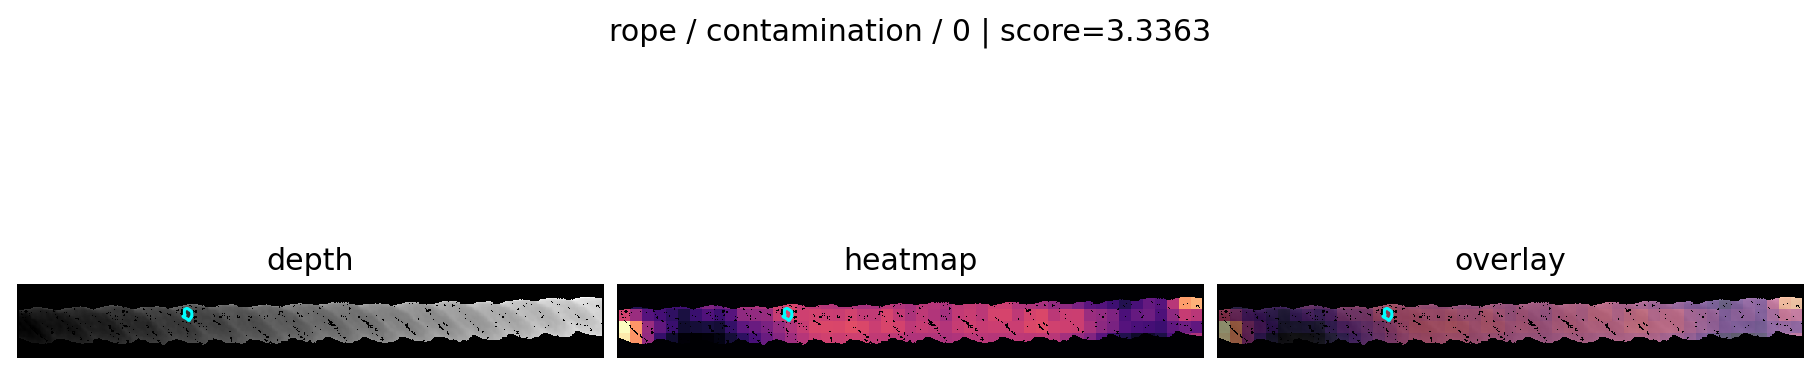
\includegraphics[width=\columnwidth]{figures/rope_contamination_heatmap.png}
    \caption{Qualitative output for a rope contamination sample. Left: processed depth map. Middle: normalized anomaly heatmap from aggregated One-Class SVM patch scores. Right: heatmap overlaid on depth. Cyan contours show the transformed ground-truth defect mask.}
    \label{fig:rope-heatmap}
\end{figure}

\subsection*{RGB investigation}
Because some defects are difficult to distinguish in depth alone, we performed a preliminary RGB signal check. RGB files are present for all $1197$ test samples, and their sizes match the ground-truth masks. This means RGB can be transformed using the same crop and resize geometry as the depth maps.

The signal check compared RGB values inside the ground-truth defect region with a local surrounding context ring. It is not a trained model, but it estimates whether color provides useful anomaly information. The strongest median RGB signal was observed for \textit{cookie} ($1.965$), \textit{potato} ($1.163$), \textit{peach} ($1.145$) and \textit{foam} ($0.998$). Particularly strong defect-type signals appeared for cookie contamination ($5.419$), cookie hole ($3.116$), potato contamination ($2.379$) and peach contamination ($2.265$). Weak signals were found for some structural or subtle cases, such as tire combined defects ($0.315$) and cable gland holes ($0.491$).

This supports a concrete adjustment to the final plan: RGB should be tested as an additional modality, especially for contamination and color-related defects, but it should not replace depth because many anomalies remain geometric or contextual.
